\chapter{Exploratory Data Analysis}
\label{sec:eda}

\section{Introdutory Data Exploration}




\begin{figure}[H]
	\caption{The three created datasets}
	\centering
	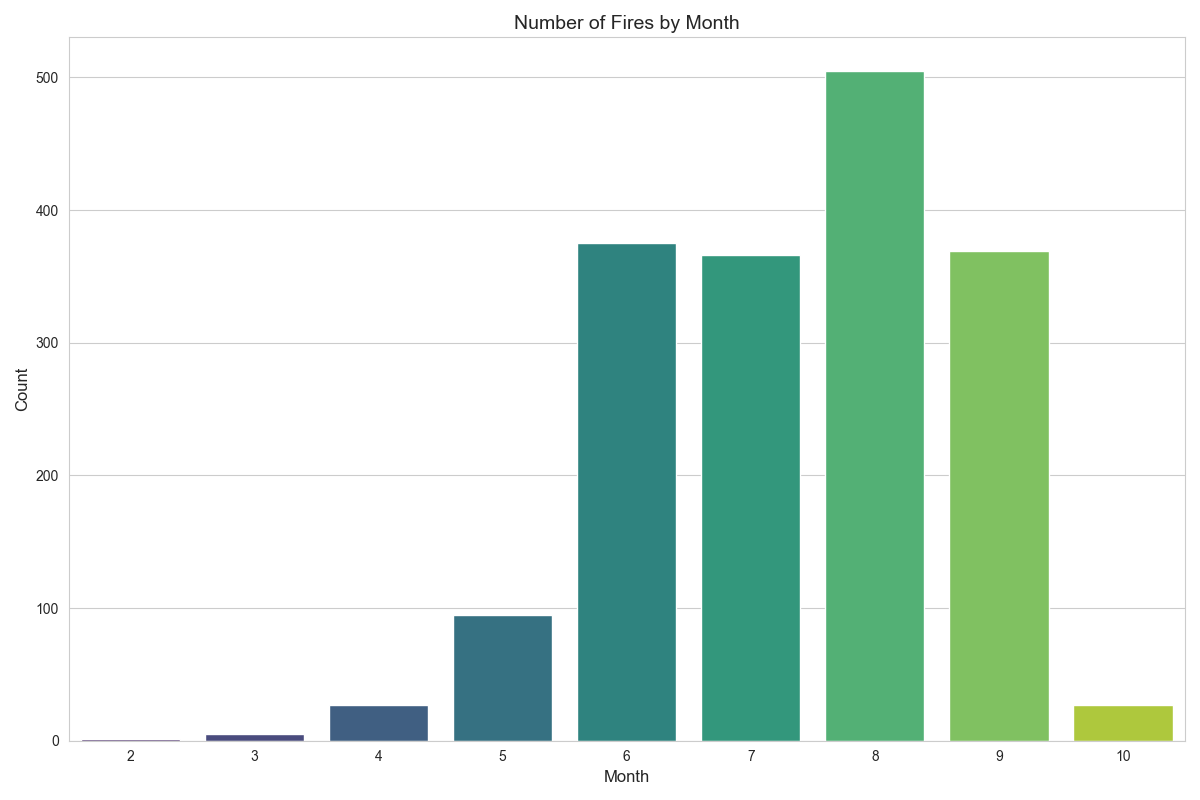
\includegraphics[width=\textwidth]{chapter-images/5_1-eda/monthly_fire_count.png}
	\label{fig:montly_fire_count}
\end{figure}



\begin{figure}[H]
	\caption{The three created datasets}
	\centering
	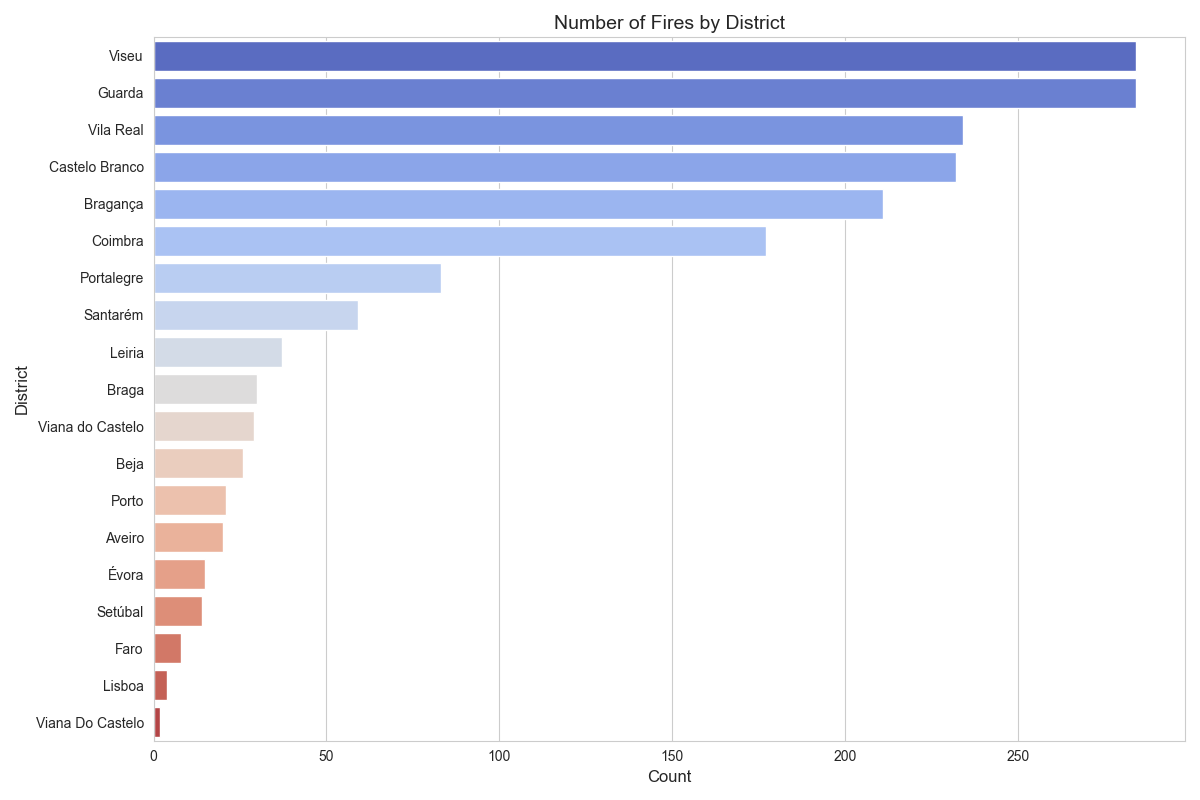
\includegraphics[width=\textwidth]{chapter-images/5_1-eda/district_fire_count.png}
	\label{fig:montly_fire_count}
\end{figure}


\subsection{Land types and Tree Species}





\cite{71c95a07-e296-44fc-b22b-415f42acfdf0}

https://land.copernicus.eu/content/corine-land-cover-nomenclature-guidelines/docs/pdf/CLC2018_Nomenclature_illustrated_guide_20190510.pdf



112 is a discontinuos urban fabric - vegetation and green spaces between buildings (gardens, lawns, flower beds, shrub and tree formations); class is assigned when urban structures and transport networks associated with vegetated areas and bare surfaces are present and occupy significant surfaces in a discontinuous spatial pattern

2 - Agricultural areas 

242 - Complex cultivation patterns. Mosaic of small cultivated land parcels with different cultivation types -annual crops, pasture and/or permanent crops-, eventually with scattered houses or gardens.

3 - Forest and seminatural areas 

324 - Transitional woodland/shrub. Transitional bushy and herbaceous vegetation with occasional scattered trees. Areas representing natural development of forest formations, consisting of young plants of broad–leaved and coniferous species, with herbaceous vegetation and dispersed solitary adult trees


these examples were taken from 

\begin{figure}[H]
	\caption{The three created datasets}
	\centering
	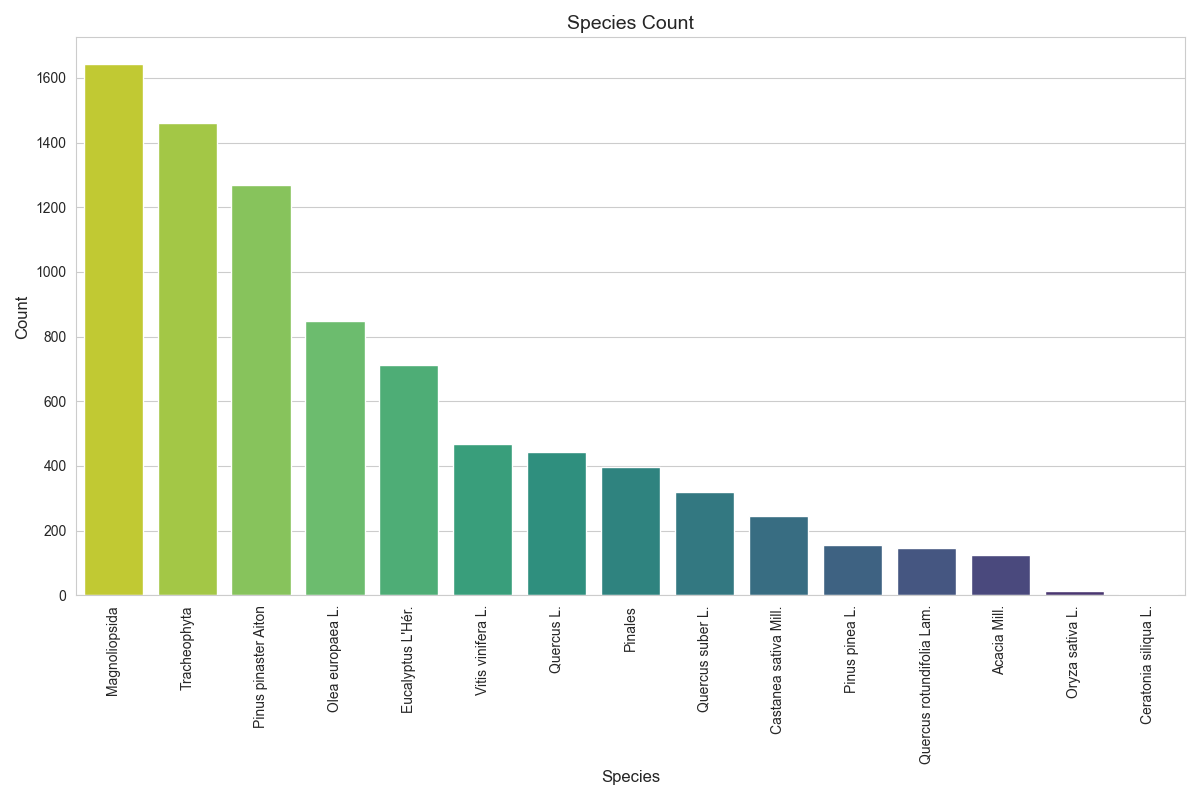
\includegraphics[width=\textwidth]{chapter-images/5_1-eda/species_count.png}
	\label{fig:species_count}
\end{figure}


\begin{figure}[H]
	\caption{Class 1.1.2 - Discontinuous urban fabric example \cite{kosztra_green_suburbs_2024}}
	\centering
	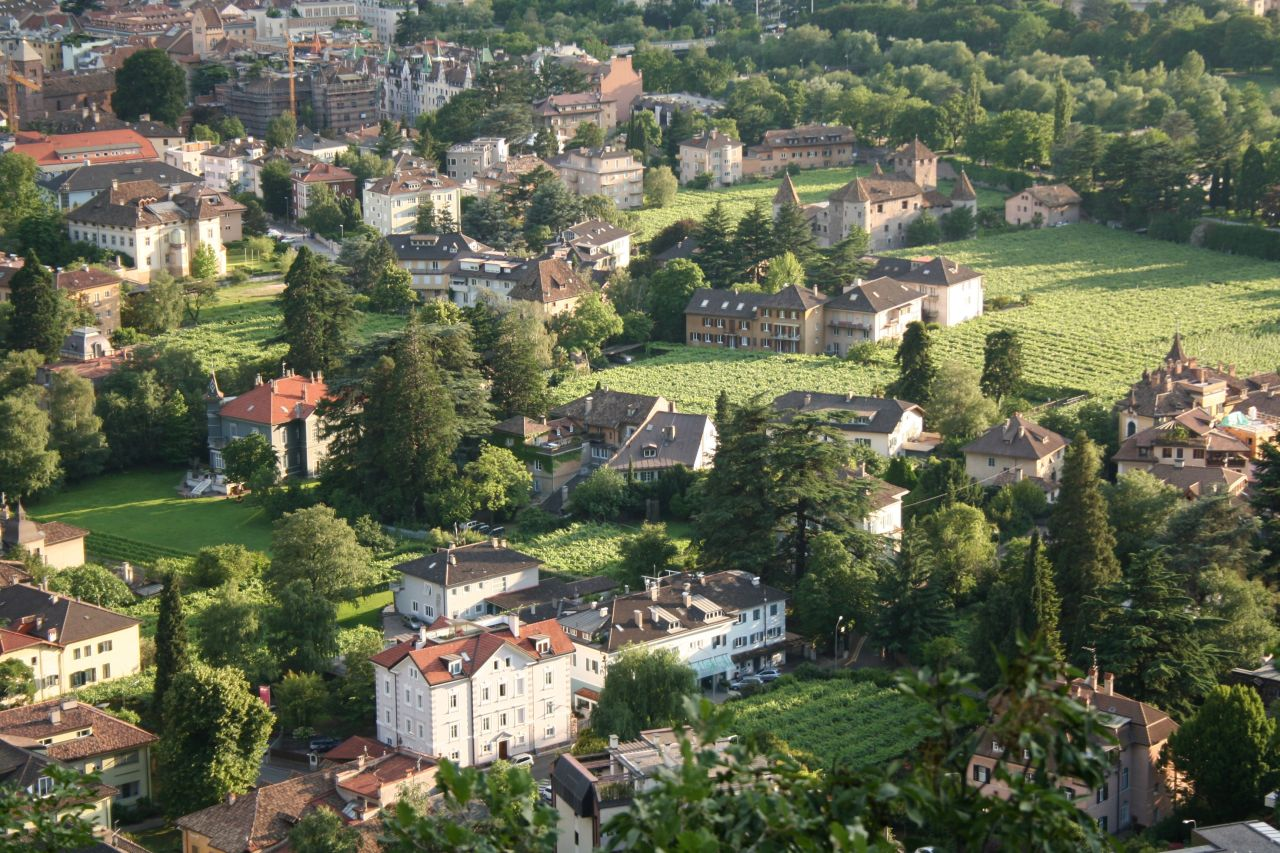
\includegraphics[width=\textwidth]{chapter-images/5_1-eda/112_IT_IMG_3074_small.jpg}
	\label{fig:species_count}
\end{figure}

\begin{figure}[H]
	\caption{Class 2.4.2 - Complex cultivation patterns example \cite{hazeu_complex_2024}}
	\centering
	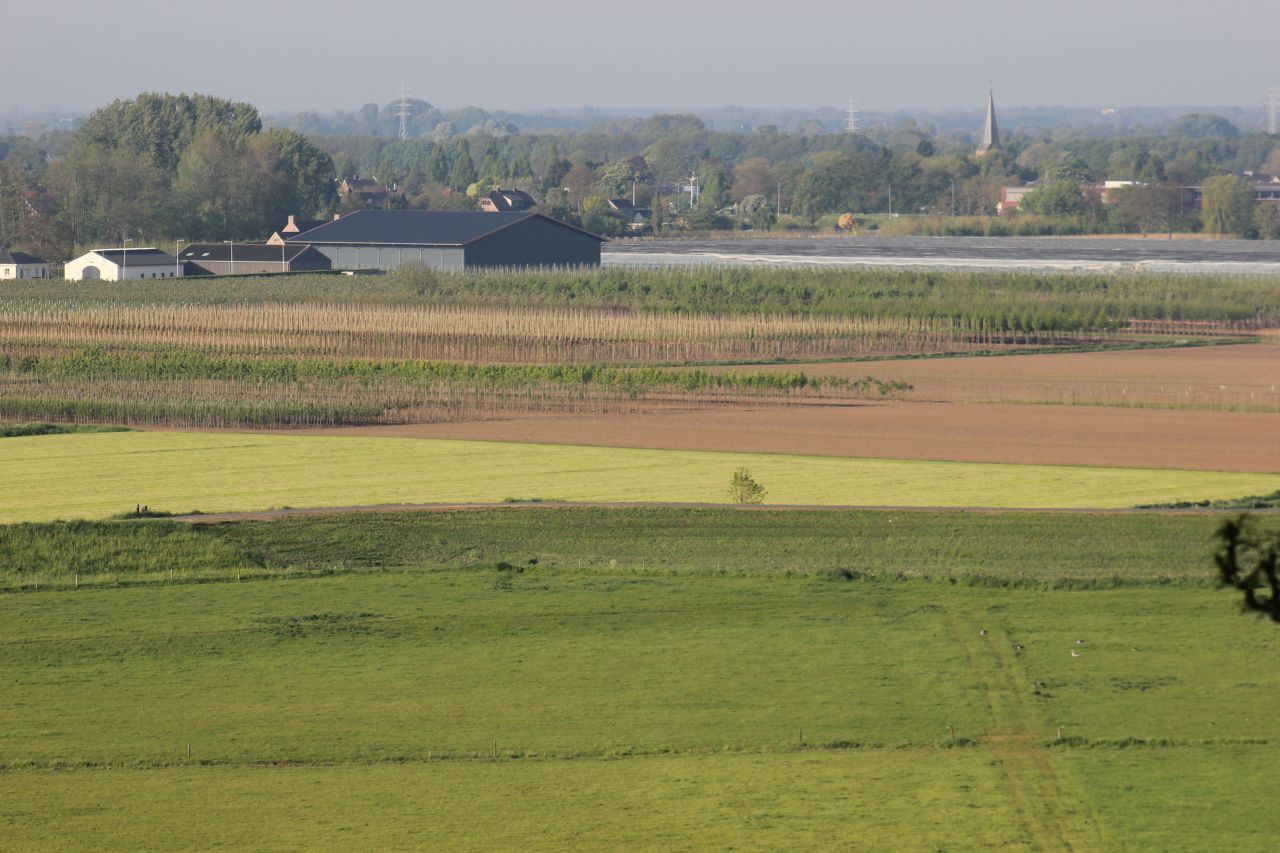
\includegraphics[width=\textwidth]{chapter-images/5_1-eda/242_NL_GH_IMG_2743_small.JPG}
	\label{fig:species_count}
\end{figure}

\begin{figure}[H]
	\caption{Class 3.2.4 - Transitional woodland/shrub example \cite{kosztra_avalanche_2024}}
	\centering
	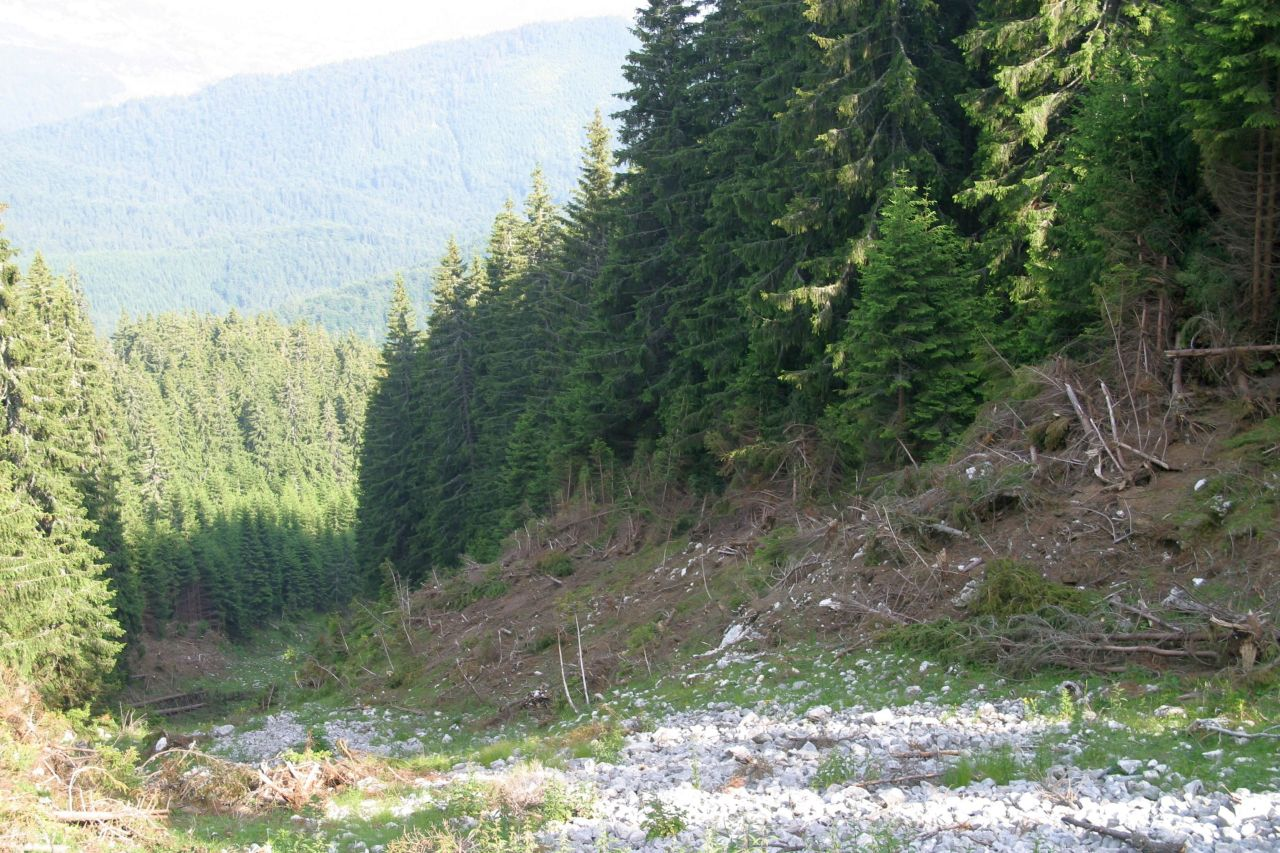
\includegraphics[width=\textwidth]{chapter-images/5_1-eda/324_RO_avalanche_damage_IMG_5664_small.jpg}
	\label{fig:species_count}
\end{figure}


\begin{figure}[H]
	\caption{The three created datasets}
	\centering
	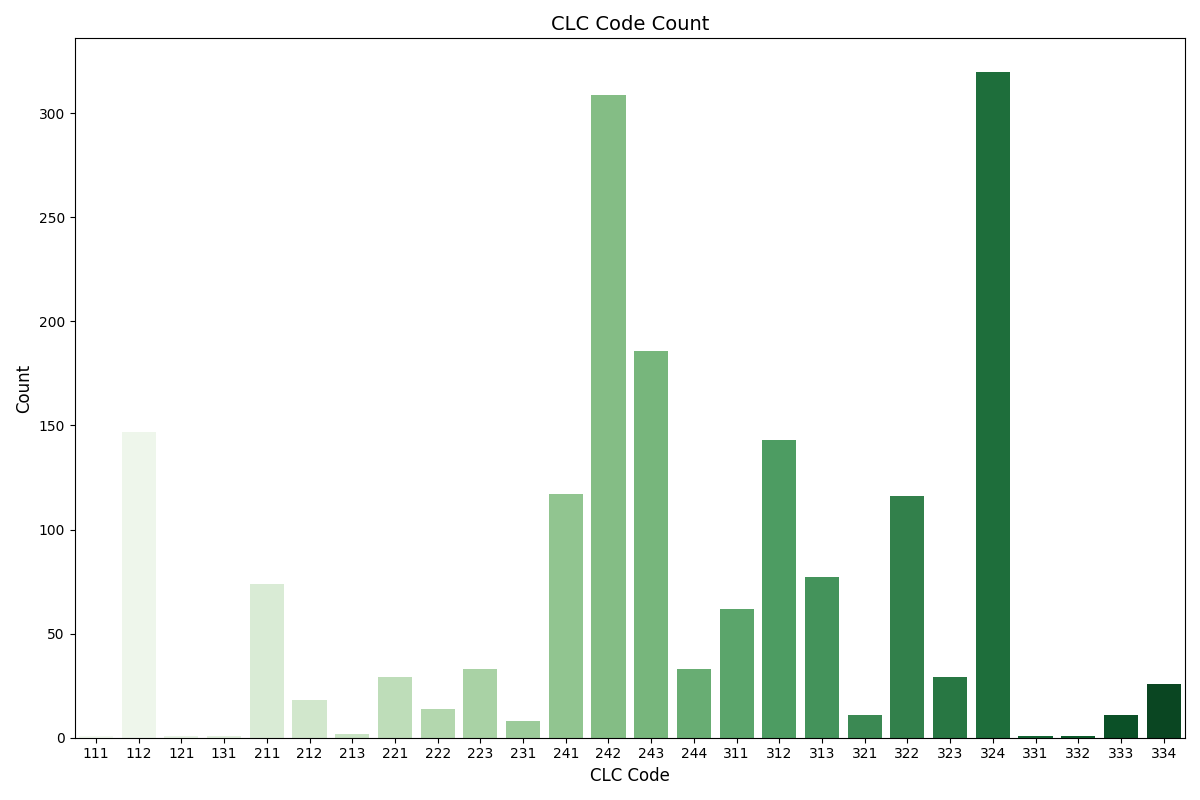
\includegraphics[width=\textwidth]{chapter-images/5_1-eda/clc_code_count.png}
	\label{fig:montly_fire_count}
\end{figure}


Portugal's vegetation is a blend of Atlantic, European, Mediterranean, and African species \cite{britannica_portugal_climate}, and four tree species account for 80\% of all the forest area: \textit{Pinus pinaster}, \textit{Eucalyptus globulus}, \textit{Quercus suber}, and \textit{Quercus rotundifolia} \cite{Marques2011}.


 




\subsection{Weather variables distribution at the time of ignition}
removed variables: 'hourly.weather\_code' 'hourly.sunshine\_duration' 'hourly.is\_day' 'hourly.snowfall',
'hourly.snow\_depth', 


\begin{figure}[H]
	\caption{The three created datasets}
	\centering
	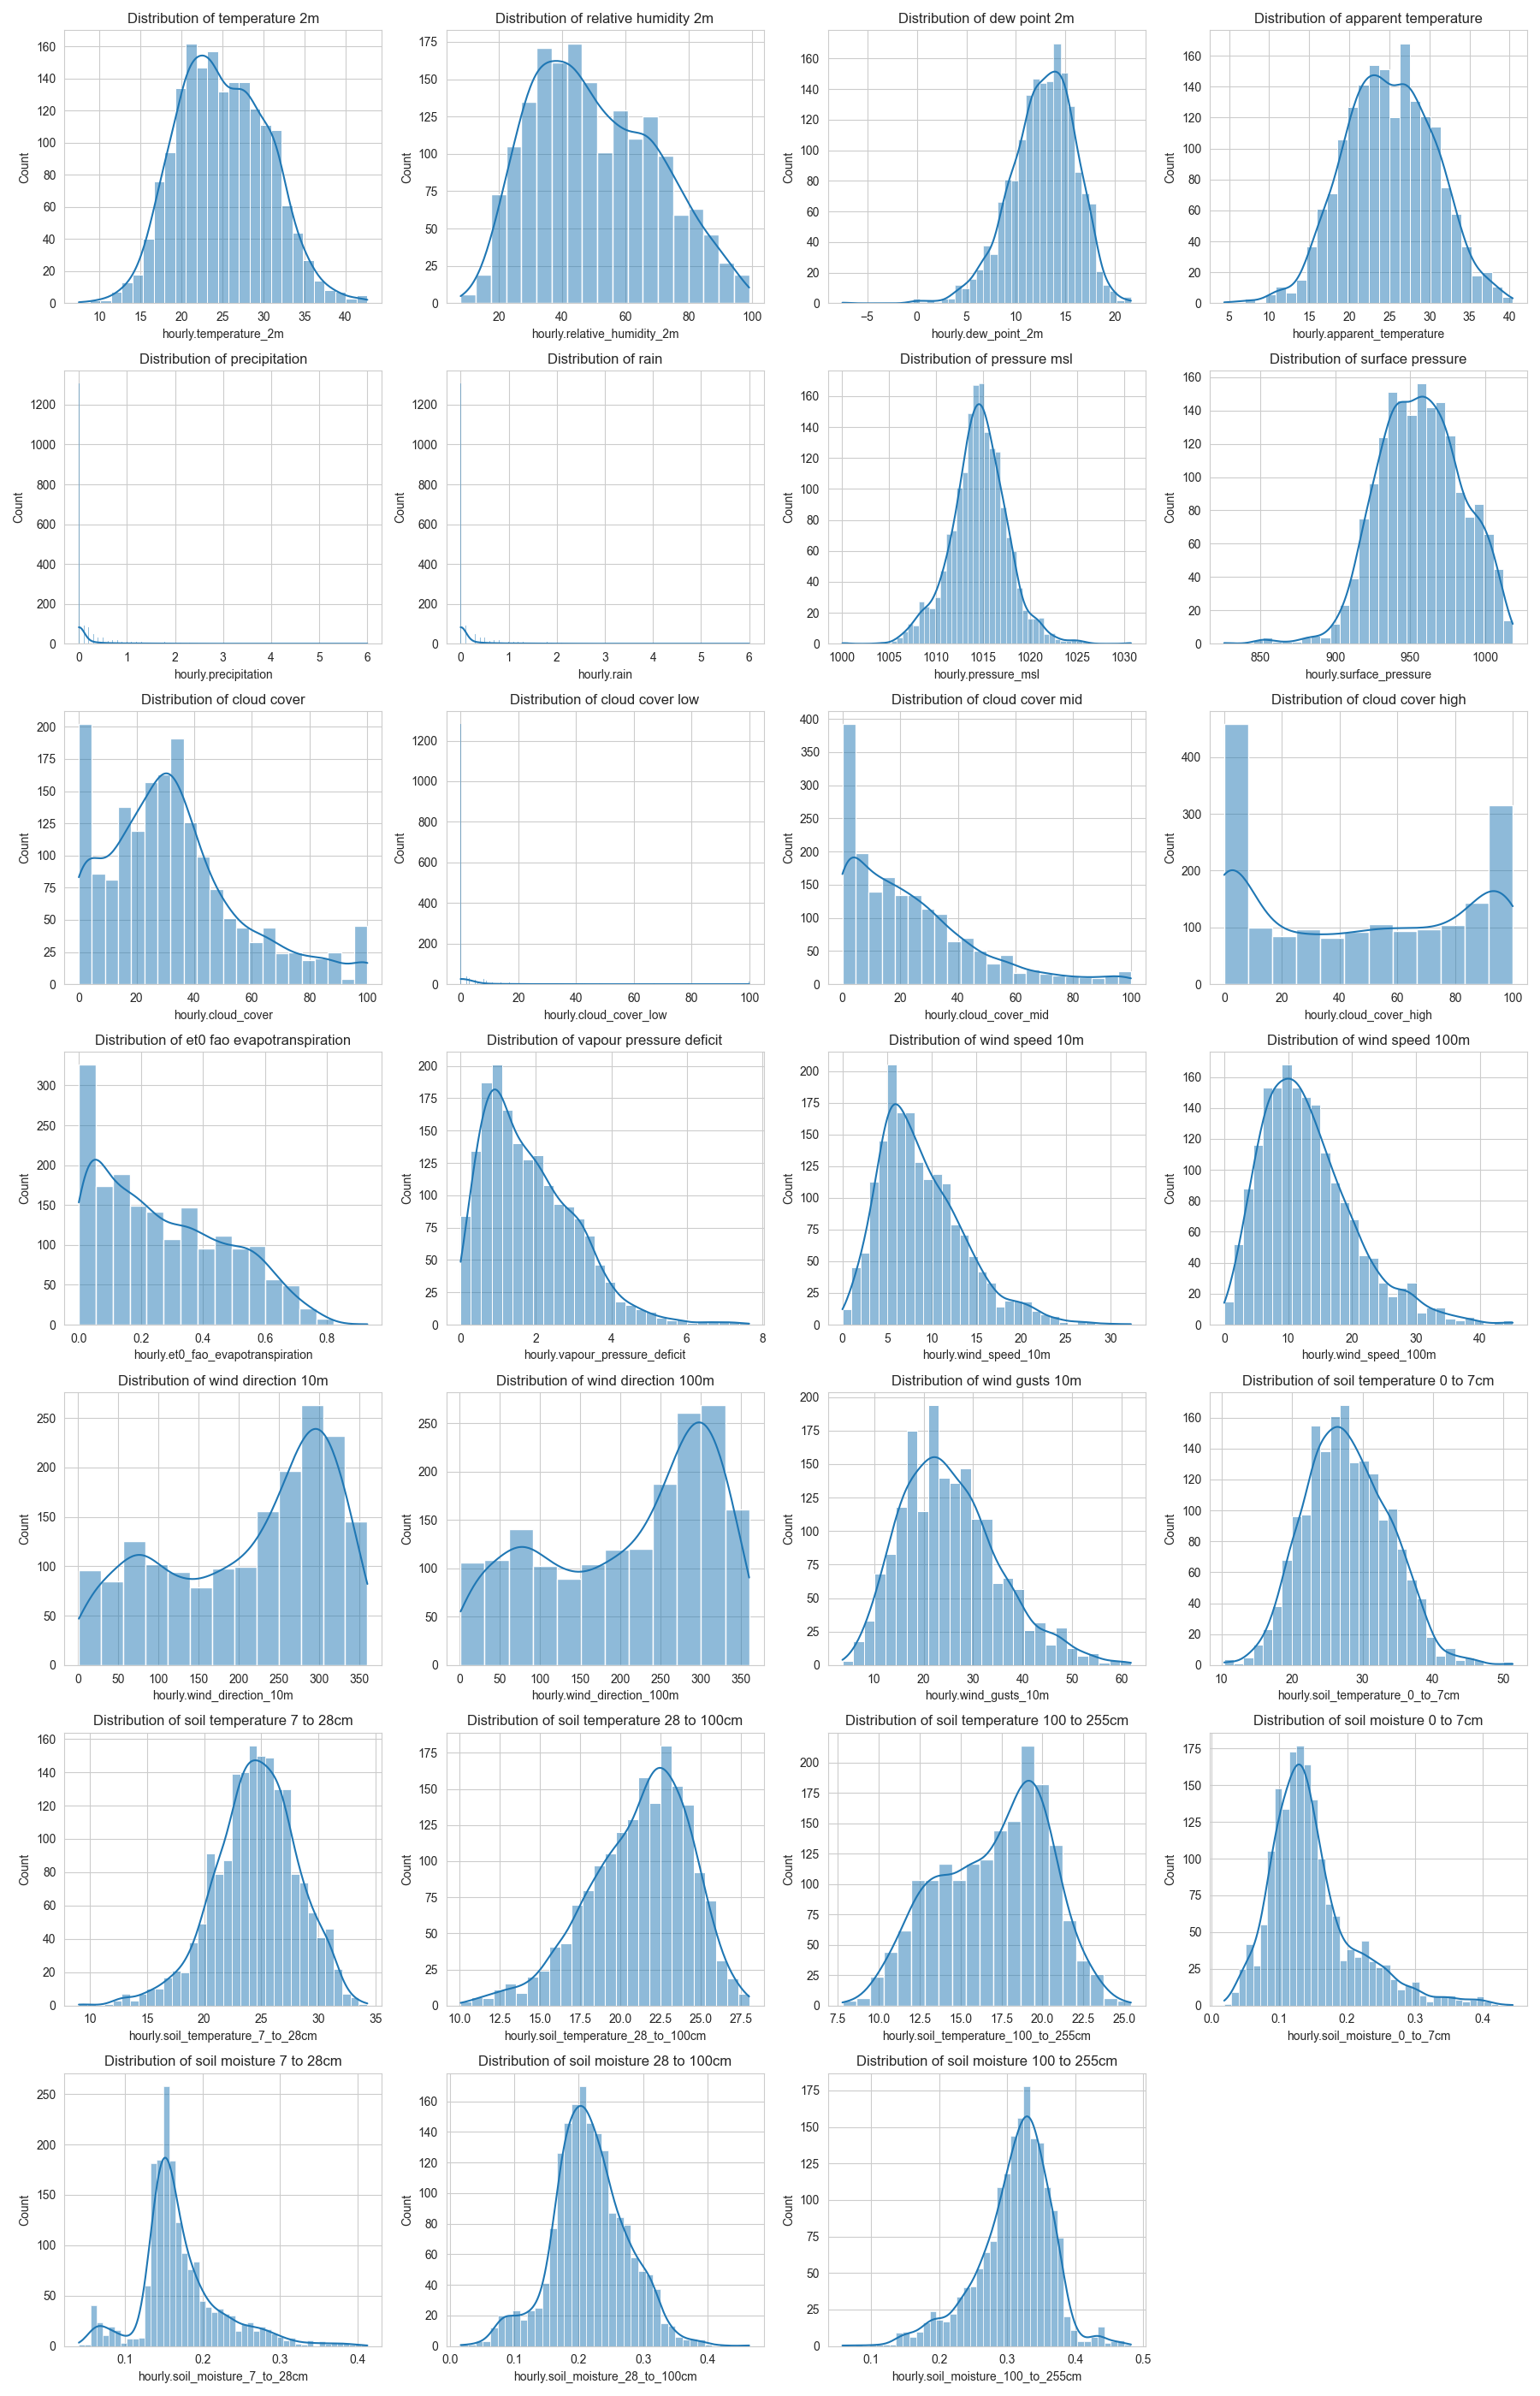
\includegraphics[width=\textwidth]{chapter-images/5_1-eda/distribution_weather_variables1FT.png}
	\label{fig:distribuiton_weather_variables}
\end{figure}

\begin{figure}[H]
	\caption{The three created datasets}
	\centering
	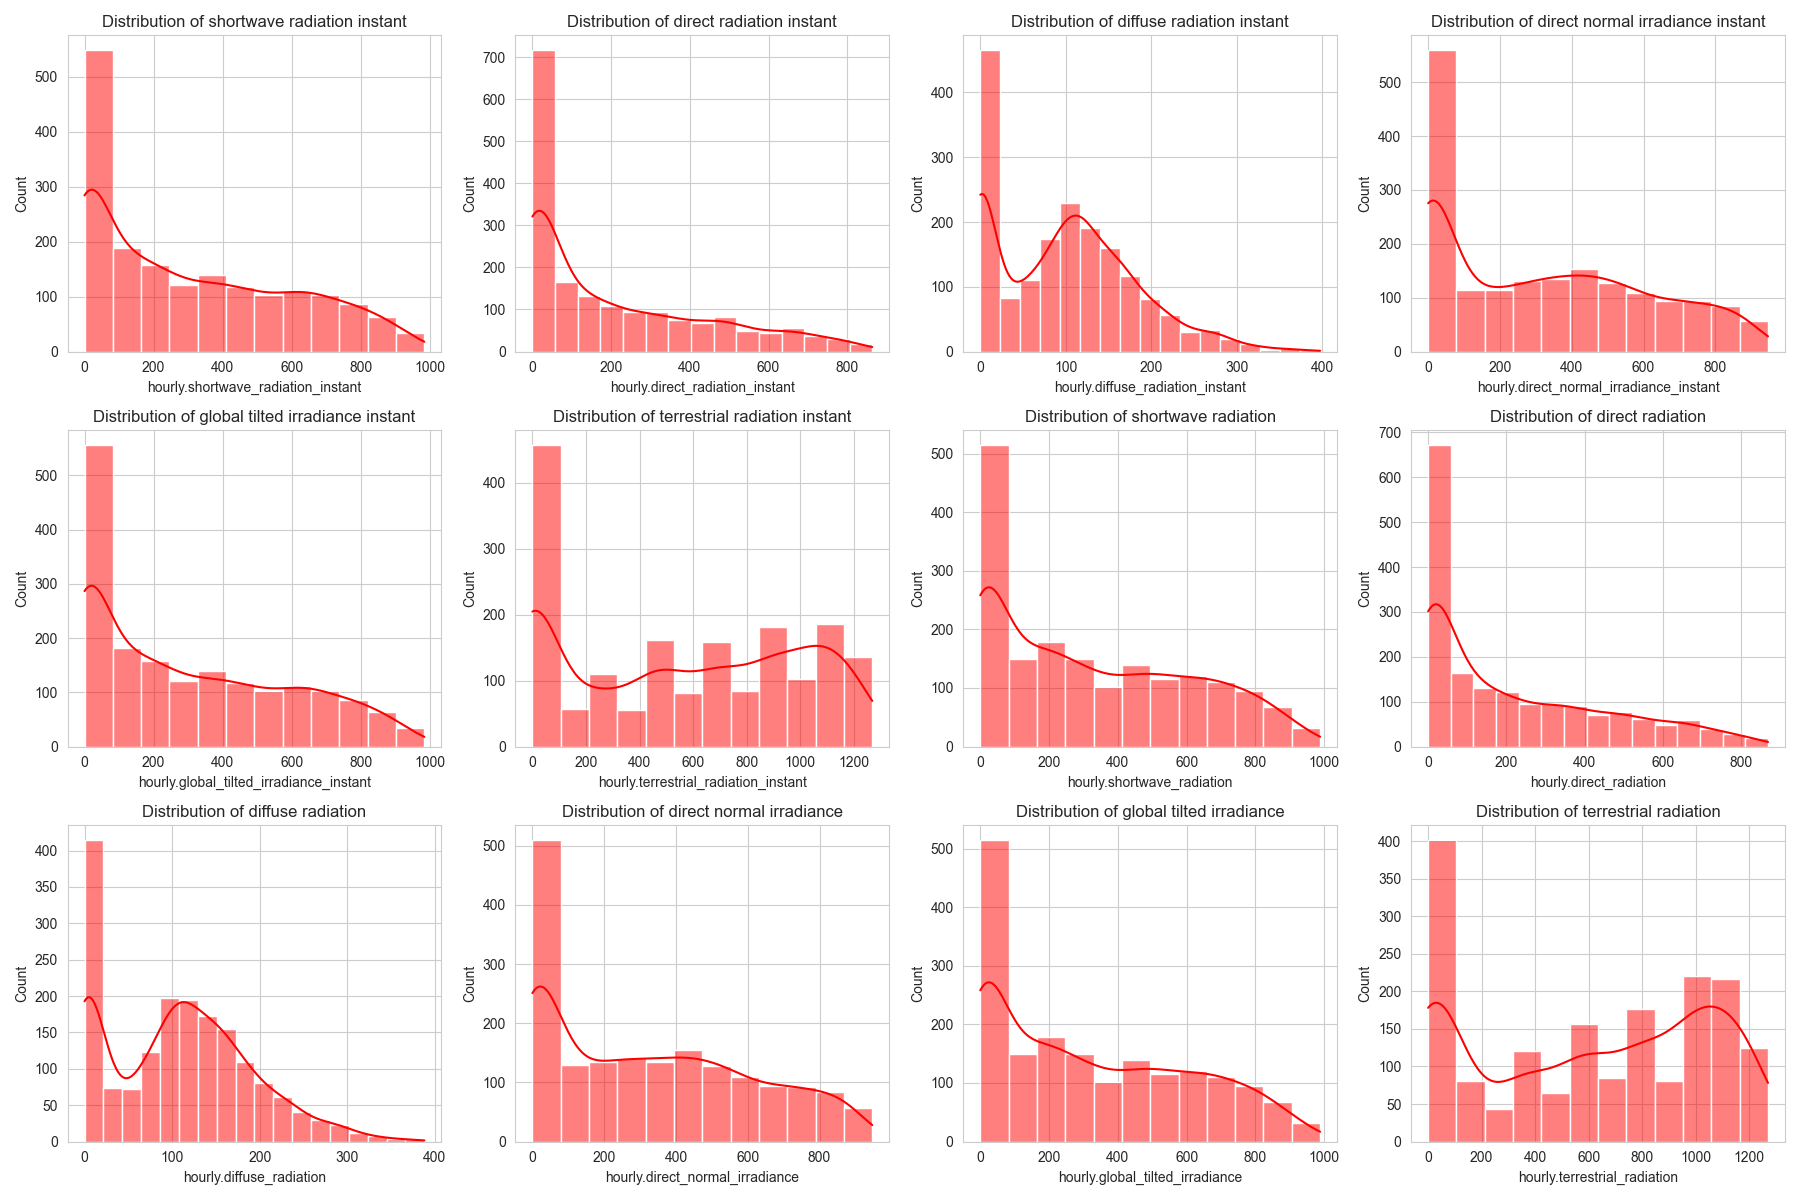
\includegraphics[width=\textwidth]{chapter-images/5_1-eda/distribution_weather_variables2FT.png}
	\label{fig:distribuiton_weather_variables_radiation}
\end{figure}







\begin{figure}[H]
	\caption{The three created datasets}
	\centering
	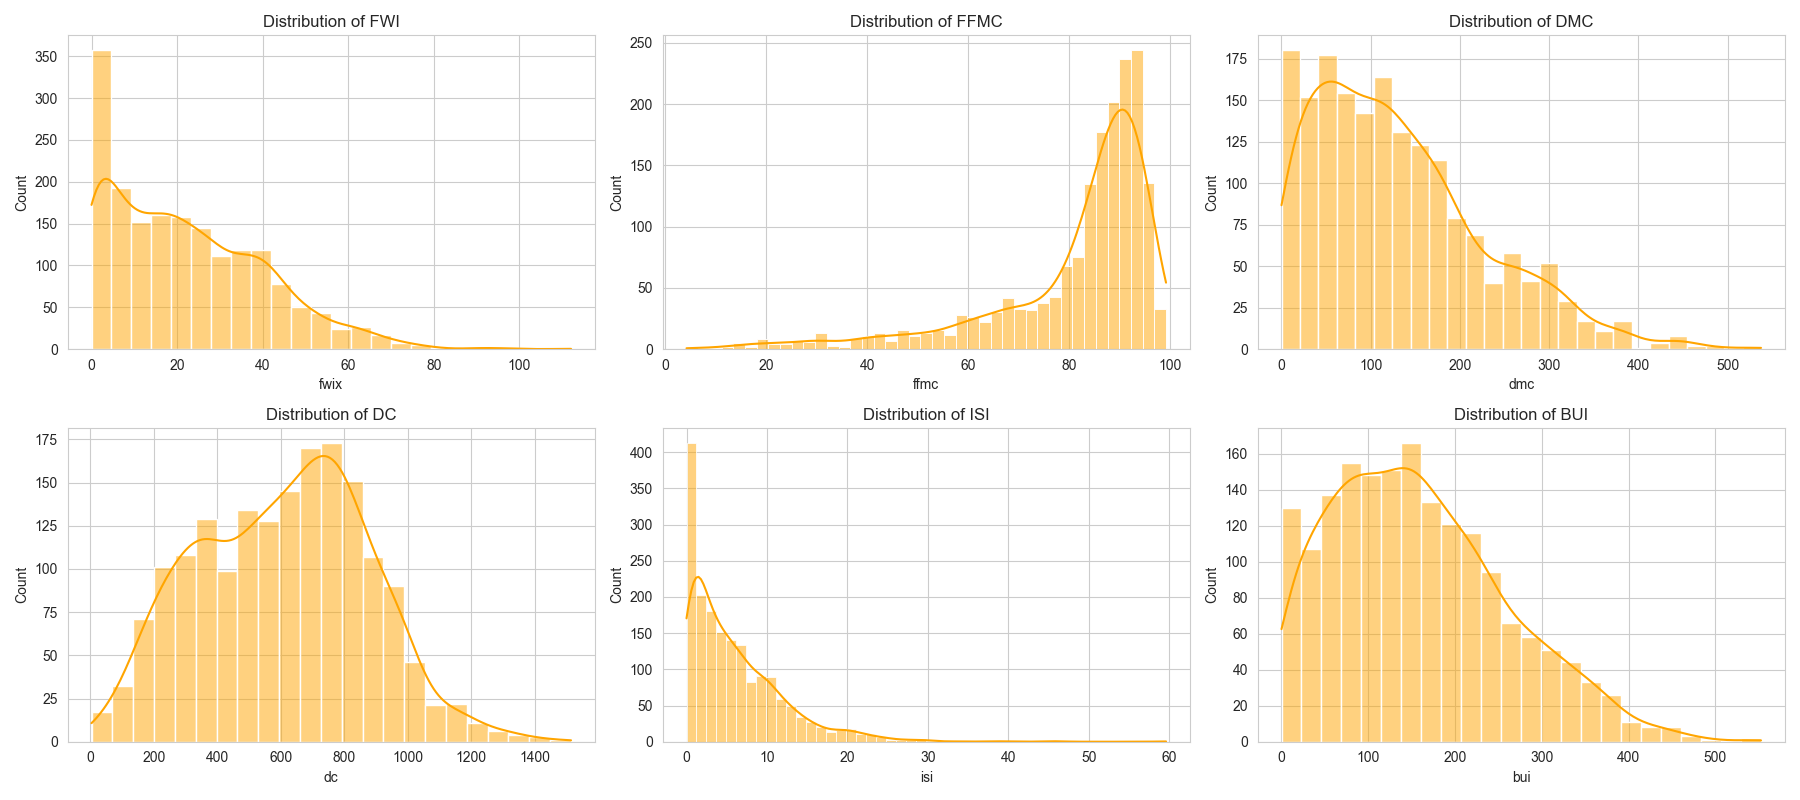
\includegraphics[width=\textwidth]{chapter-images/5_1-eda/distribution_weather_variables3FT.png}
	\label{fig:montly_fire_count}
\end{figure}

\section{Average conditions at ignition time}

\begin{table}[H]
	\centering
	\begin{tabular}{lrl}
		\toprule
		Parameter & Value & Unit \\
		\midrule
		hour &  14.6 & hours \\
		temperature\_2m & 25.06678 & °C \\
		relative\_humidity\_2m & 50.342373 & \% \\
		dew\_point\_2m & 12.720565 & °C \\
		apparent\_temperature & 24.98887 & °C \\
		precipitation & 0.180847 & mm \\
		rain & 0.180847 & mm \\
		snowfall & 0.0 & cm \\
		snow\_depth & 0.0 & meters \\
		pressure\_msl & 1014.581243 & hPa \\
		surface\_pressure & 956.793955 & hPa \\
		cloud\_cover & 32.822599 & \% \\
		cloud\_cover\_low & 5.60904 & \% \\
		cloud\_cover\_mid & 23.429379 & \% \\
		cloud\_cover\_high & 47.100565 & \% \\
		et0\_fao\_evapotranspiration & 0.271921 & mm \\
		vapour\_pressure\_deficit & 1.831282 & kPa \\
		wind\_speed\_10m & 8.881864 & km/h \\
		wind\_speed\_100m & 13.092881 & km/h \\
		wind\_direction\_10m & 212.215254 & ° \\
		wind\_direction\_100m & 209.636158 & ° \\
		wind\_gusts\_10m & 25.422655 & km/h \\
		soil\_temperature\_0\_to\_7cm & 27.828192 & °C \\
		soil\_temperature\_7\_to\_28cm & 24.509492 & °C \\
		soil\_temperature\_28\_to\_100cm & 21.176949 & °C \\
		soil\_temperature\_100\_to\_255cm & 17.014124 & °C \\
		soil\_moisture\_0\_to\_7cm & 0.148219 & $m^3/m^3$ \\
		soil\_moisture\_7\_to\_28cm & 0.171308 & $m^3/m^3$ \\
		soil\_moisture\_28\_to\_100cm & 0.216619 & $m^3/m^3$ \\
		soil\_moisture\_100\_to\_255cm & 0.310751 & $m^3/m^3$ \\
		\bottomrule
	\end{tabular}
	\caption{Hourly Weather Data with Units}
	\label{tab:hourly_weather_data_units}
\end{table}


\begin{table}[H]
	\centering
	\begin{tabular}{lrl}
		\toprule
		Parameter & Value & Unit \\
		\midrule
		shortwave\_radiation\_instant & 308.195706 & $W/m^2$ \\
		direct\_radiation\_instant & 209.089096 & $W/m^2$ \\
		diffuse\_radiation\_instant & 99.105367 & $W/m^2$ \\
		direct\_normal\_irradiance\_instant & 324.071525 & $W/m^2$ \\
		global\_tilted\_irradiance\_instant & 307.808701 & $W/m^2$ \\
		terrestrial\_radiation\_instant & 563.058305 & $W/m^2$ \\
		shortwave\_radiation & 328.19435 & $W/m^2$ \\
		direct\_radiation & 220.187006 & $W/m^2$ \\
		diffuse\_radiation & 108.007345 & $W/m^2$ \\
		direct\_normal\_irradiance & 330.480113 & $W/m^2$ \\
		global\_tilted\_irradiance & 328.19435 & $W/m^2$ \\
		terrestrial\_radiation & 610.627627 & $W/m^2$ \\
		roughness & 178.799333 & - \\
		aspect & 178.957915 & ° \\
		slope & 8.162517 & ° \\
		mean\_elev & 36.125026 & meters \\
		fwi & 22.317299 & - \\
		ffmc & 81.146887 & - \\
		dmc & 130.720423 & - \\
		dc & 606.997705 & - \\
		isi & 6.064164 & - \\
		bui & 158.466257 & - \\
		\bottomrule
	\end{tabular}
	\caption{Hourly Weather Data with Units}
	\label{tab:hourly_weather_data_units}
\end{table}






